% !TEX TS-program = pdflatex
% !TEX encoding = UTF-8 Unicode
% !TEX root = ../practice2.tex
% !TEX spellcheck = en-CA

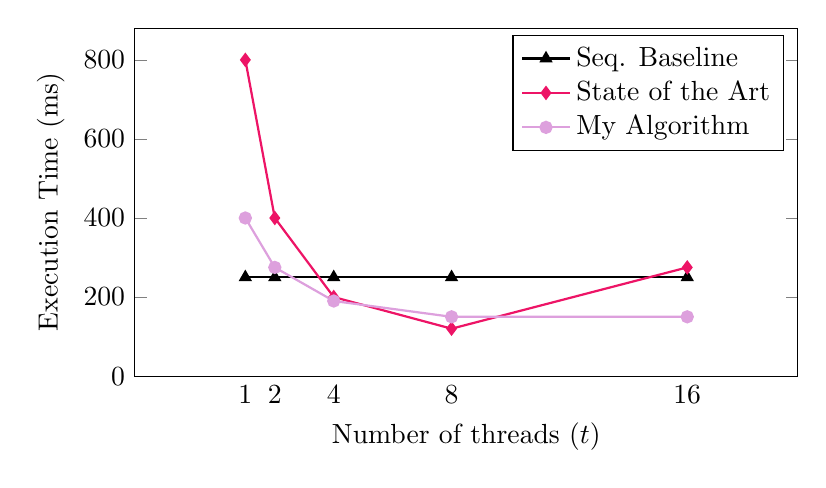
\begin{tikzpicture}
    \begin{axis}[
        height = 6cm,
        width = 10cm,
        major x tick style = transparent,
%        extra y ticks={0,200,400,600,800,1000},
        ymin = 0,
        xlabel = {Number of threads ($t$)},
        ylabel = {Execution Time (ms)},
        xtick = data,
        scaled y ticks = true,
        enlarge x limits=0.25,
        legend cell align=left,
        legend columns=1,
    ]

        \addplot[thick,mark size=2,color=black,mark=triangle*]
             coordinates {(1,250) (2,250) (4,250) (8,250) (16,250)};
	   \addlegendentry{Seq. Baseline}
             
        \addplot[thick,mark size=2,color=WildStrawberry,mark=diamond*]
            coordinates {(1, 800) (2,400) (4,200) (8,120) (16,275)};
	   \addlegendentry{State of the Art}
             
        \addplot[thick,mark size=2,color=Plum,mark=*]
            coordinates {(1, 400) (2,275) (4,190) (8,150) (16,150)};
	   \addlegendentry{My Algorithm}

    \end{axis}
\end{tikzpicture}
